\documentclass[a4paper, 12pt]{article}
\usepackage{bm}
\usepackage{amssymb}
\usepackage{graphicx}
\usepackage{amsmath}
\usepackage{breqn}
\usepackage{amsfonts}
\usepackage{float}
\usepackage{wrapfig}
\graphicspath{ {images/} }
\begin{document}
\begin{center} 
{\Huge{\textbf{Instantons}}}\\
\end{center}

\section {What are Instantons?}
Instantons refer to localised finite-action solutions of the classical Euclidean equation of motion that connects two potential maxima. They are in some sense similar to solitons but instead they are localised in time. 
\section {How to get Euclidean action?}
To go from Minkowsi space to Euclidean space we do the analytic continuation of time, i.e. t$\to -i\tau$, this is also called \textbf{Wick rotation}. The Euclidean action is defined as
\begin{equation}
S_{Euc} = -i(S_{Min})_{continued}
\end{equation}
As an example let's see the Minkowski Klien-Gordon system. The action is 
\begin{equation}
S_{Min} = \int dt \int dx \bigg[\frac{1}{2}\bigg(\frac{\partial\phi}{\partial t} \bigg)^2 - \frac{1}{2}(\nabla \phi)^2 -m^2 \phi^2  \bigg],
\end{equation}
which yields the field equation
\begin{equation}
\bigg( \frac{\partial^2}{\partial t^2} - \nabla^2 \bigg)\phi + m^2\phi = 0.
\end{equation}
So doing the processes mentioned above, we get that
\begin{equation}%%%%%%%%%%%%% 4 %%%%%%%%%%%%%%%
S_{Euc} = \int dx_4 \int dx \bigg[\frac{1}{2}\bigg(\frac{\partial\phi}{\partial x_4} \bigg)^2 + \frac{1}{2}(\nabla \phi)^2 + m^2 \phi^2  \bigg]
\end{equation}
which yields the field equation
\begin{equation}%%%%%%%%%%%%% 5 %%%%%%%%%%%%%%%
\bigg( \frac{\partial^2}{\partial {x_4}^2} + \nabla^2 \bigg)\phi - m^2\phi = 0.
\end{equation}
Since we can write the path integral as
\begin{equation}%%%%%%%%%%%%% 6 %%%%%%%%%%%%%%%
G(q_i,q_f;t) = \int Dq \*\ \textrm{exp}\bigg[\frac{i}{\hbar}S_{Min}\bigg] =  \int Dq \*\ \textrm{exp}\bigg[\frac{i}{\hbar}\int_0^t dt \bigg(\frac{m}{2}\dot{q^2} - V(q) \bigg) \bigg]
\end{equation}
In the imaginary time we can also write this as
\begin{equation}%%%%%%%%%%%%% 7 %%%%%%%%%%%%%%%
G_E(q_i,q_f;\tau) = \int Dq \*\ \textrm{exp}\bigg[-\frac{1}{\hbar}S_{Euc}\bigg] =  \int Dq \*\ \textrm{exp}\bigg[-\frac{1}{\hbar}\int_0^\tau d\tau' \bigg(\frac{m}{2}\dot{q^2} + V(q) \bigg) \bigg].
\end{equation}
One can see that the potential V becomes -V. We can see the same thing from the stationary phase equations
\begin{equation}
-m\ddot{q} + V'(q) = 0.
\end{equation}

Some important observations:
\begin{itemize}
\item Minkowski energy $\equiv$ Euclidean action.
\item The Euclidean action is like static soliton solutions in higher dimensions.
\item  Like the finiteness of energy of solitons, here we have finiteness of Euclidean action. From the path-integral representation we can see that if action is infinite it leads to zero contribution.
\end{itemize}


Before looking into the instanton problem we first need to see the semiclassics from the path integral.


\section {Semiclassics from path integral}

The general functional integral we have is of the form $\int Dx $ $e^{-F[x]}$. We use the stationary phase approximation and do the taylor series expansion of the functional. To get the stationary path we minimize the functional and get the classical path.
\begin{equation}
\frac{\delta F[x]}{\delta x(t)} \Bigg|_{x=\bar{x}} = 0.
\end{equation}
Now we Taylor expand the functional to second order around $\bar{x}$, i.e.
\begin{equation}
F[x] = F[\bar{x}+y] = F[\bar{x}] + \frac{1}{2}\int dt \int dt' y(t')A(t,t')y(t) + ... ,
\end{equation}
where $A(t,t') = \frac{\delta^2 F[x]}{\delta x(t) \delta x(t')} \bigg|_{x=\bar{x}}$ denotes the second functional derivative.\\
If the operator $\hat{A} \equiv \{A(t,t')\}$ is positive definite, then the functional integration reduces to
\begin{equation}
\int Dx \*\ e^{-F[x]} \simeq \sum_i e^{-F[\bar{x}_i]} \*\ \textrm{det}\bigg(\frac{\hat{A}_i}{2\pi}\bigg)^{-1/2}.
\end{equation}
Putting the lagrangian as $L(q,\dot{q}) = m\dot{q}^2/2 - V(q)$, we get the second functional derivative as:
\begin{equation}
 \frac{1}{2}\int dt \int dt' r(t')A(t,t')r(t) =  -\frac{1}{2}\int dt  r(t')[m\partial^2_t + V''(q_{cl})]r(t).
\end{equation}
As an example of the above let's see a quantum particle in a well. Let the well be centred around $q=0$. Let's evaluate G(0,0;t), minimising the action gives the classical path as $q_{cl}(t)=0$ whoch then further gives $S[q_{cl}(t)]=0$. On expanding the potential we get, $V''(q)= m\omega^2$. This gives the transition amplitude as
\begin{equation}
G(0,0;t) \simeq \int Dr \*\ \textrm{exp} \bigg[-\frac{i}{\hbar}\int_0^t dt'  r(t')\frac{m}{2}(\partial^2_{t'} + \omega^2)]r(t')\bigg].
\end{equation}
This integral gives us
\begin{equation} %%%%%%%%%%%%% 14 %%%%%%%%%%%%%%%
G(0,0;t) \simeq J \textrm{det}(-m(\partial^2_{t} + \omega^2)/2)^{-1/2}
\end{equation}
Finding the eigenvalues and then evaluating the determinant gives us
\begin{equation} %%%%%%%%%%%%% 15 %%%%%%%%%%%%%%%
G(0,0;t) \simeq J \sqrt{\frac{m\omega}{2\pi i \hbar \textrm{sin}(\omega t)}} \*\ \Theta(t).
\end{equation}
The above expression is exact for harmonic oscillator. We will now use this tool to evaluate the double well potential.

\section {Double well potential: tunneling and instantons}
\begin{figure}[ht]
    \centering
    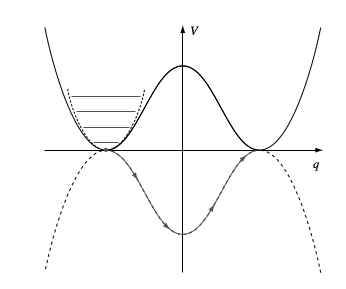
\includegraphics[height=5cm, width=6cm]{fig1}
\end{figure}

Our aim is to estimate the probability amplitude that particle stays at one minima or tunnels from one to the other minima. Using the Euclidean path integral formulation the transition amplitude is given by
\begin{equation}%%%%%%%%%%%%% 16 %%%%%%%%%%%%%%%
G_E(a,\pm a;\tau)=  \int_{q(0)=\pm a}^{q(\tau)=a} Dq \*\ \textrm{exp}\bigg[-\frac{1}{\hbar}\int_0^\tau d\tau' \bigg(\frac{m}{2}\dot{q^2} + V(q) \bigg) \bigg].
\end{equation}
If the particle stays in one of the minima it's the same as the expression (15). Now the interesting stuff happens when the particle tunnels. Let's first see the classical solution of this problem. For that we minimise the action that then gives us that energy of the classical particle should be constant. Now since in Euclidean time formalism we replace V by -V. Also when the particle is at the boundaries the enrgy is 0. This gives us
\begin{equation}
\frac{m}{2}\dot{q}^2_{cl}=V(q_{cl}).
\end{equation}
This gives the instanton action as
\begin{equation}
S_{inst} = \int_0^{\tau} d\tau ' m\dot{q}^2_{cl} = \int  d\tau ' \frac{dq_{cl}}{dt}(m\dot{q}) = \int_{-a}^{a} dq (2mV(q))^{1/2}.
\end{equation}
Defining the second of potential at $\pm a$ by $V(\pm a)=m\omega^2$, equation (17) then implies, $\dot{q}= -\omega(q_{cl}-a)$ (for the particle close to the right maximum). This equation then integrates to $\lim{\tau \to \infty} q_{cl} \to a - e^{-\tau \omega}$. We see that the classical action depends only on the potential and it does not care about the path $q_{cl}$.\\
\begin{figure}[ht]
    \centering
    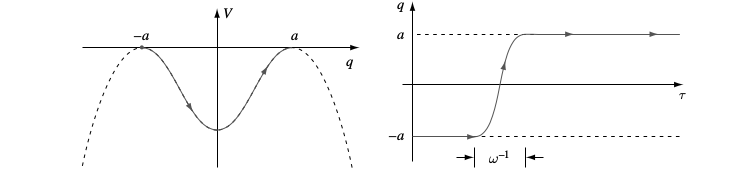
\includegraphics[height=4cm, width=15cm]{fig2}
\end{figure}

There are two important things to note:
\begin{itemize}
\item The solution is confined to a narrow interval of time. So there must exist approximate solutions of the stationary equation involving firther instanton/anti-instanton pairs.
\item Acoording to saddle-point scheme, the path integral is obtained by summing over all solutions(see (11)) of saddle point equations and hence over all instanton configurations. The summation over multi-instanton configuration is referred to as \textbf{``instanton gas"}.
\end{itemize}
Since the instantons have short temporal support we can take the dilute gas approximation or that the two instantons don't overlap or the overlap contribution is very small. So for multi-instanton configuration we can write
\begin{equation}
G(a,\pm a; \tau) \simeq \sum_{n\*\ \mathrm{even/odd}}K^n \int_0^{\tau}d\tau_1 \int_0^{\tau_1}d\tau_2 ... \int_0^{\tau_{n-1}}d\tau_n \*\ A_n(\tau_1,...,\tau_n),
\end{equation}
where $A_n$ denotes the amplitude associated with n instantons, and we have taken into account that even/odd for $\pm a$. Here K denotes a constant absorbing the temporal dimensions.
\begin{figure}[ht]
    \centering
    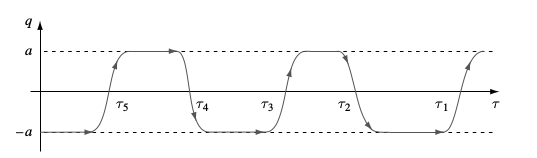
\includegraphics[height=4cm, width=15cm]{fig3}
\end{figure}

Now, $A_n = A_{n,cl} \times A_{n,qu} $, where the terms show the classical and quantum contributions respectively. So we can write
\begin{equation}
A_{n,cl}(\tau_1,...,\tau_n) = e^{-nS_{inst}/\hbar},
\end{equation}
which is independent of the time coordinates $\tau_i$. For finding $ A_{n,qu} $ we notice that the quantum fluctuation of the single instanton is given in equation (15), we just need to move it to imaginary time($t \to -i\tau$). So it simplifies as
\begin{equation}
\sqrt{\frac{1}{\mathrm{sin}(-i\omega(\tau_{i+1}-\tau_{i}))}} \sim e^{-\omega(\tau_{i+1}-\tau_{i})/2},
\end{equation}
which gives
\begin{equation}
A_{n,qu}(\tau_1,...,\tau_n) = e^{-\omega\tau /2}.
\end{equation}
This implies
\begin{dmath}
G(a,\pm a; \tau) \simeq \sum_{n\*\ \mathrm{even/odd}}K^n e^{-nS_{inst}/\hbar}e^{-\omega\tau /2}\int_0^{\tau}d\tau_1 \int_0^{\tau_1}d\tau_2 ... \int_0^{\tau_{n-1}}d\tau_n  = e^{-\omega\tau /2} \sum_{n\*\ \mathrm{even/odd}}\frac{1}{n!}\Big(K \tau e^{-S_{inst}/\hbar}\Big)^n .
\end{dmath}
Performing the summation gives
\begin{dmath}
G(a,\pm a; \tau) \simeq Ce^{-\omega\tau /2} \mathrm{cosh}\Big(K \tau e^{-S_{inst}/\hbar}\Big),
\\ \*\ Ce^{-\omega\tau /2} \mathrm{sinh}\Big(K \tau e^{-S_{inst}/\hbar}\Big)
\end{dmath}
where C is some factor not depending exponentially on time. To find the average or effective number of instantons contributing to the sum we calculate $\langle n \rangle \equiv \Sigma_n c_n n/ \Sigma_n c_n$ (define X $\equiv \tau K e^{-S_{inst}/\hbar}$)
\begin{equation}
\langle n \rangle \equiv \frac{\Sigma_n nX^n/n!}{\Sigma_n X^n/n!} = X.
\end{equation}
We see that $\langle n \rangle /\tau = K e^{-S_{inst}/\hbar}$, that is the average instanton density is independent of $\tau$ and is exponentially small compared to instanton action, validating our dilute gas assumption.\\
Thinking in physical terms we know that degeneracy is lifted from the two states due to overlap or tunneling. For a weak inter-barrier coupling, the ground states split into a symmetric and anti-symmetric eigenstates $|S\rangle$ and $|A \rangle$, with energies $\epsilon_S$ and $\epsilon_A$.
\begin{equation}
G(a,\pm a;\tau) \simeq \langle a| \bigg( |S\rangle e^{-\epsilon_S \tau /\hbar} \langle S| + |A\rangle e^{-\epsilon_A \tau /\hbar} \langle A|   \bigg) |\pm a\rangle.
\end{equation}
This gives $\epsilon_{A/S}=\hbar \omega /2 \pm \Delta \epsilon /2$ where $\Delta \epsilon$ represents the tunnel-splitting.
\begin{figure}[ht]
    \centering
    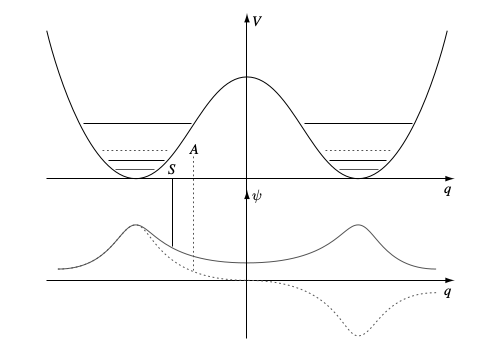
\includegraphics[height=6cm, width=8cm]{fig4}
\end{figure}

The instanton calculation gives us that the tunnel splitting of energies,
\begin{equation}
\Delta \epsilon = \hbar K \*\ \mathrm{exp}(-S_{inst}/\hbar)
\end{equation}
which upto a constant agrres with the WKB-result for tunneling processes. The value of K is given as
\begin{equation}
K = \bigg| {\frac{\overline{S_{inst}}}{2\pi \hbar}} \frac{\mathrm{det}[-\partial_t^2 + \omega^2]}{\mathrm{det'}[-\partial_t^2 + V''(\bar{x})]}\bigg|^{\frac{1}{2}}
\end{equation}
\\
\section {Escape from metastable minimum: bounces}


\begin{figure}[ht]
    \centering
    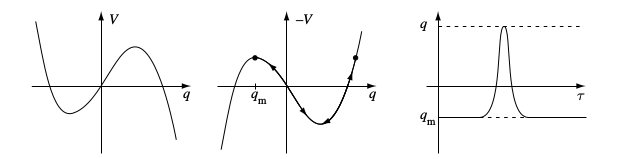
\includegraphics[height=4cm, width=15cm]{fig5}
\end{figure}

If we want to calculate the survival probability, the probability amplitude of remaining at the potential minimum $q_m$. The classical solution here takes the form of a \textbf{``bounce''}. Similar to the instanton we can expect multiple bounce trajectories to give significant contribution. Summing over all the trajectories here gives the survival probability as
\begin{equation}
G(q_m,q_m;\tau) = Ce^{-\omega\tau /2} \mathrm{exp}\Big(K \tau e^{-S_{bounce}/\hbar}\Big)
\end{equation}
Doing the analytic continuation gives $G(q_m,q_m;t) = Ce^{-i\omega t /2} \mathrm{exp}\big[-\frac{\Gamma}{2}t\big]$ where the decay rate is given by $\Gamma /2 = |K| e^{-S_{bounce}/\hbar}$.(On physical grounds we see that K must be imaginary.)
\section {Periodic instantons}

\section {Tunneling of quantum fields}

%%%%\begin{figure}[ht]
%%%%    \centering
%%%%    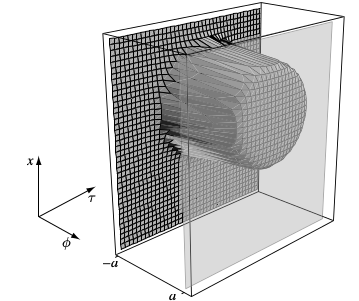
\includegraphics[height=9cm, width=9cm]{fig6}
%%%%\end{figure}

  \section {References}
1. Solitons and Instantons by R. Rajaraman.\\
2. Aspects of Symmetry by Sidney Coleman.\\
3. Condensed Matter Field Theory by Altland and Simons.





\end{document}